\documentclass{../../text-style}

\texttitle{Практика по многопоточному программированию}

\begin{document}

\maketitle
\thispagestyle{empty}

\section{Разбор домашки, или о замере времени работы программы}

В домашней работе про перемножение матриц был намеренно провокационный пункт условия про то, что надо сравнить скорость работы последовательного и пралаллельного алгоритмов. Подавляющее большинство решений использовало Stopwatch, в вызовы которого оборачивало последовательное решение, параллельное, а потом просто печатало на экран результаты.

Это вообще не показательно. Если бы вы запустили программу несколько раз, вы бы увидели, что времена получаются каждый раз разные. Более того, в тех решениях, которые честно перебирали размеры матриц и количество потоков, было видно, что сначала времена работы ведут себя ожидаемо, но с ростом количества потоков начинают вести себя странно, то увеличиваясь, то уменьшаясь. Хорошо, что никто не сделал вывод, что идеально 25 потоков, потому что там наименьшее время достигается, но с такими экспериментальными данными могли бы.

Дело в том, что вообще физическое время работы программы определяется массой случайных факторов, например, общей загрузкой процессора и системы в целом (у вас может внезапно запуститься фоновый процесс по обновлению Windows, например), тактовой частотой процессора (любой современный процессор имеет переменную частоту для экономии электроэнергии, и управляет ей, как ему заблагорассудится), капризами планировщика, погодой на Марсе. Кроме того, есть ещё разрешение системного таймера (обычно это единицы миллисекунд), мерять временные промежутки меньше этой величины просто нельзя, как должны были объяснять на уроках физики в седьмом классе. Да и просто указыввать временные промежутки в миллисекундах можно только для сравнения и для иллюстрации, потому что на других машинах и даже на другой ОС и даже на другой версии .NET время работы может быть совсем другим. К счастью, в домашке в эту ловушку никто не попал, но иметь это в виду надо.

Как делать правильно --- использовать матстат (который вам пока не рассказывали, но некоторое интуитивное представление, думаю, у всех есть). Время работы программы --- это всегда некоторая случайная величина, а измерения времени --- это выборка из этой величины, по которой нам надо определить её параметры (представьте, например, самолёт, который мы раз в секунду наблюдаем на радаре с некоторой погрешностью и нам надо оценить реальную траекторию его полёта --- мы никогда не можем сделать это точно из-за погрешности, но мы можем сказать, что с такой-то вероятностью он движется вот так). Время работы имеет чаще всего нормальное распределение (также известное как распределеине Гаусса), по смыслу оно устроено так, что большинство значений сконцентрированы вокруг среднего, но могут быть выбросы, но чем они больше, тем менее вероятны. 

Нормальное распределение характеризуется двумя параметрами --- матожиданием и дисперсией (либо среднеквадратическим отклонением --- это просто корень из дисперсии, но его легче понять). Матожидание --- это просто среднее значение (то есть если взять достаточно большую выборку и усреднить, получим примерно матожидание), дисперсия --- это разброс величины относительно матожидания (то есть, насколько можно доверять измерениям). Если дисперсия мала, то мы можем померять величину достаточно точно (если меньше разрешения таймера, то максимально возможно точно). Если же дисперсия велика, величина ведёт себя очень хаотично и матожидание нам мало что даёт (например, если среднеквадратичное отклонение больше матожидания, то измерения вообще бессмысленны, мы не можем предсказать даже примерно время следующего запуска программы). 

Задача эксперимента --- по набору измерений определить матожидание и дисперсию случайной величины с приемлемой точностью. Как это делать правильно, расскажут на матстате, для начала сойдёт так: запускаем десять раз программу (а лучше сто), получаем $T_1$, ..., $T_n$ измерений времени. Считаем среднее (по формуле $E = \frac{\sum_{i = 1}^{n}T_i}{n}$) --- это оценка матожидания. Дальше считаем среднее квадратов разницы матожидания и значений (по формуле $D = \frac{\sum_{i = 1}^{n}(E - T_i)^2}{n}$, квадрат там только для того, чтобы отрицательные отклонения вносили положительный вклад, так что формула только выглядит страшной) --- это оценка дисперсии. Корень из неё --- это средний разброс измерений. Если он выглядит приличным, то радуемся, если нет, пытаемся понять, то ли мы вообще мерим и правильно ли это делаем. И вот именно эти результаты (матожидание и дисперсия) и являются результатами замеров, никак не время одного запуска в миллисекундах! Кстати, обратите внимание, что матожидание измеряется в миллисекундах, дисперсия --- в миллисекундах в квадрате.

Это касается не только этой домашки, но и любых замеров вообще. Говорить что-то о случайной величине по одному замеру --- верный способ отправиться пересдавать учебную практику, например.

\section{Напоминание про условия взаимной блокировки}

Взаимоблокировка (Deadlock) --- это когда N потоков ждут друг друга и ни один из них не может продвинуться, потому что чтобы работать, ему нужно, чтобы отработал кто-то другой. Блокировка возникает тогда, когда:

\begin{enumerate}
    \item имеется разделяемый ресурс (например, файл), к которому потоки хотят получить доступ, но пользоваться им может только один поток, и пока он им пользуется, другие не могут его получить;
    \item таких ресурсов несколько и поток, захватив один, хочет получить доступ к другим (или другому), которые в этот момент захвачены другими потоками;
    \item нельзя отнять захваченный ресурс у потока;
    \item потоки ждут друг друга <<по кругу>> --- один ждёт ресурс, захваченный вторым, второй --- третьим, третий --- ..., N-й --- первым, и так как никто не может продолжить свою работу и отдать захваченный им ресурс, вся работа стоит, вечно.
\end{enumerate}

Блокировка возможна, только когда выполнены сразу все эти условия, так что её можно избежать, нарушив хотя бы одно из них.

Рекомендую посмотреть визуализации в английской википедии\footnote{Deadlock, URL: \url{https://en.wikipedia.org/wiki/Deadlock}, дата обращения: 31.08.2020)}.

\section{Задача}

Собственно, чтобы попробовать руками ситуацию блокировки и как её избежать, предлагается на паре просимулировать известную задачу <<обедающих философов>>:

\begin{itemize}
    \item есть N тарелок спагетти, N вилок и N философов;
    \item каждый философ может думать и есть, больше он ничего не делает;
    \item чтобы есть, философу нужны две вилки (в оригинале философы ели рис палочками, но что-то пошло не так);
    \item когда философ думает, просто ничего не происходит, когда он проголодается, он пытается взять вилки и, если ему удалось, начинает есть, ест некоторое время, кладёт вилки и продолжает думать;
    \item если вилки взять не удалось, философ ждёт и пытается таки поесть, если представится возможность.
\end{itemize}

Вот картинка, визуализирующая происходящее:

\begin{center}
    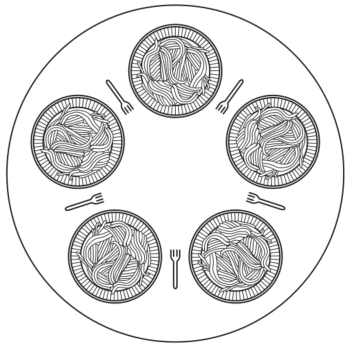
\includegraphics[width=0.5\textwidth]{diningPhilosophers.png}
    \attribution{A. Tanenbaum, Modern Operating Systems}
\end{center}

Пример ситуации обедающих философов в реальной жизни --- это банковские транзакции. Допустим, вы хотите заплатить за телефон, ваш друг хочет перевести вам деньги, и он работает в телефонной компании, которая в этот же момент хочет заплатить ему зарплату. Чтобы выполнить перевод, надо залочить два счёта, но если каждая транзакция залочит один счёт и будет ждать, пока отдадут другой --- случится печаль.

Что хочется сделать:

\begin{itemize}
    \item придумать объектно-ориентированную модель для симуляции задачи. Философ --- независимая свободно мыслящая сущность, поэтому по идее каждый философ должен жить в своём потоке, где он попеременно думает и ест;
    \item для синхронизации философы используют вилки, отдельный класс для них не нужен, потому что вилки ничем друг от друга не отличаются, но при желании можно сделать;
    \item надо выводить на экран состояния философов --- что он хочет есть, взял одну вилку и готовится взять другую, взяд две вилки и ест, закончил есть и положил вилки; следует также печатать номера вилок;
    \item считаем, что философы думают и едят случайное, но небольшое количество времени;
    \item реализация должна гарантировать отсутствие взаимоблокировок. Точнее, надо сначала сделать наивное решение, добиться того, чтобы философы мешали друг другу, а затем придумать алгоритм, который позволяет блокировок избежать;
    \item как только блокировок не будет, надо задуматься о том, как корректно останавливать процесс и распускать философов по домам. Просто прерывать работу нельзя, иначе какой-нибудь философ может не доесть, надо, чтобы все философы закончили есть, увидели, что всё закончилось и вышли из своих циклов, и только после этого программа завершала бы работу.
\end{itemize}

\end{document}
